\documentclass{beamer}
\usepackage{amsmath}
\usepackage[english]{babel} %set language; note: after changing this, you need to delete all auxiliary files to recompile
\usepackage[utf8]{inputenc} %define file encoding; latin1 is the other often used option
\usepackage{csquotes} % provides context sensitive quotation facilities
\usepackage{graphicx} %allows for inserting figures
\usepackage{booktabs} % for table formatting without vertical lines
\usepackage{textcomp} % allow for example using the Euro sign with \texteuro
\usepackage{stackengine}
\usepackage{wasysym}
\usepackage{tikzsymbols}
\usepackage{textcomp}
\usepackage{ragged2e} % para alinear
\usepackage{graphicx}  % Para incluir imágenes
\usepackage{tikz}  
\usepackage{booktabs}
\usepackage{colortbl}
\usepackage{xcolor}
\usepackage{array}
\usepackage{wrapfig}
% ELIMINAR COMANDOS DE NAVEGACION%%%%%%%%%%%
\setbeamertemplate{navigation symbols}

%\newcommand{\bubblethis}[2]{
 %       \tikz[remember picture,baseline]{\node[anchor=base,inner sep=0,outer sep=0]%
 %       (#1) {\underline{#1}};\node[overlay,cloud callout,callout relative pointer={(0.2cm,-0.7cm)},%
 %       aspect=2.5,fill=yellow!90] at ($(#1.north)+(-0.5cm,1.6cm)$) {#2};}%
 %   }%
%\tikzset{face/.style={shape=circle,minimum size=4ex,shading=radial,outer sep=0pt,
 %       inner color=white!50!yellow,outer color= yellow!70!orange}}

%% Some commands to make the code easier
\newcommand{\emoticon}[1][]{%
  \node[face,#1] (emoticon) {};
  %% The eyes are fixed.
  \draw[fill=white] (-1ex,0ex) ..controls (-0.5ex,0.2ex)and(0.5ex,0.2ex)..
        (1ex,0.0ex) ..controls ( 1.5ex,1.5ex)and( 0.2ex,1.7ex)..
        (0ex,0.4ex) ..controls (-0.2ex,1.7ex)and(-1.5ex,1.5ex)..
        (-1ex,0ex)--cycle;}
\newcommand{\pupils}{
  %% standard pupils
  \fill[shift={(0.5ex,0.5ex)},rotate=80] 
       (0,0) ellipse (0.3ex and 0.15ex);
  \fill[shift={(-0.5ex,0.5ex)},rotate=100] 
       (0,0) ellipse (0.3ex and 0.15ex);}

\newcommand{\emoticonname}[1]{
  \node[below=1ex of emoticon,font=\footnotesize,
        minimum width=4cm]{#1};}
\usepackage{scalerel}
\usetikzlibrary{positioning}
\usepackage{xcolor,amssymb}
\newcommand\dangersignb[1][2ex]{%
  \scaleto{\stackengine{0.3pt}{\scalebox{1.1}[.9]{%
  \color{red}$\blacktriangle$}}{\tiny\bfseries !}{O}{c}{F}{F}{L}}{#1}%
}
\newcommand\dangersignw[1][2ex]{%
  \scaleto{\stackengine{0.3pt}{\scalebox{1.1}[.9]{%
  \color{red}$\blacktriangle$}}{\color{white}\tiny\bfseries !}{O}{c}{F}{F}{L}}{#1}%
}
\usepackage{fontawesome} % Social Icons
\usepackage{epstopdf} % allow embedding eps-figures
\usepackage{tikz} % allows drawing figures
\usepackage{amsmath,amssymb,amsthm} %advanced math facilities
\usepackage{lmodern} %uses font that support italic and bold at the same time
\usepackage{hyperref}
\usepackage{tikz}
\hypersetup{
    colorlinks=true,
    linkcolor=blue,
    filecolor=magenta,      
    urlcolor=blue,
}
\usepackage{tcolorbox}
%add citation management using BibLaTeX
\usepackage[citestyle=authoryear-comp, %define style for citations
    bibstyle=authoryear-comp, %define style for bibliography
    maxbibnames=10, %maximum number of authors displayed in bibliography
    minbibnames=1, %minimum number of authors displayed in bibliography
    maxcitenames=3, %maximum number of authors displayed in citations before using et al.
    minnames=1, %maximum number of authors displayed in citations before using et al.
    datezeros=false, % do not print dates with leading zeros
    date=long, %use long formats for dates
    isbn=false,% show no ISBNs in bibliography (applies only if not a mandatory field)
    url=false,% show no urls in bibliography (applies only if not a mandatory field)
    doi=false, % show no dois in bibliography (applies only if not a mandatory field)
    eprint=false, %show no eprint-field in bibliography (applies only if not a mandatory field)
    backend=biber %use biber as the backend; backend=bibtex is less powerful, but easier to install
    ]{biblatex}
\addbibresource{../mybibfile.bib} %define bib-file located one folder higher


\usefonttheme[onlymath]{serif} %set math font to serif ones

\definecolor{beamerblue}{rgb}{0.2,0.2,0.7} %define beamerblue color for later use

%%% defines highlight command to set text blue
\newcommand{\highlight}[1]{{\color{blue}{#1}}}


%%%%%%% commands defining backup slides so that frame numbering is correct

\newcommand{\backupbegin}{
   \newcounter{framenumberappendix}
   \setcounter{framenumberappendix}{\value{framenumber}}
}
\newcommand{\backupend}{
   \addtocounter{framenumberappendix}{-\value{framenumber}}
   \addtocounter{framenumber}{\value{framenumberappendix}}
}

%%%% end of defining backup slides

%Specify figure caption, see also http://tex.stackexchange.com/questions/155738/caption-package-not-working-with-beamer
\setbeamertemplate{caption}{\insertcaption} %redefines caption to remove label "Figure".
%\setbeamerfont{caption}{size=\scriptsize,shape=\itshape,series=\bfseries} %sets figure  caption bold and italic and makes it smaller


\usetheme{Boadilla}

%set options of hyperref package
\hypersetup{
    bookmarksnumbered=true, %put section numbers in bookmarks
    naturalnames=true, %use LATEX-computed names for links
    citebordercolor={1 1 1}, %color of border around cites, here: white, i.e. invisible
    linkbordercolor={1 1 1}, %color of border around links, here: white, i.e. invisible
    colorlinks=true, %color links
    anchorcolor=black, %set color of anchors
    linkcolor=beamerblue, %set link color to beamer blue
    citecolor=blue, %set cite color to beamer blue
    pdfpagemode=UseThumbs, %set default mode of PDF display
    breaklinks=true, %break long links
    pdfstartpage=1 %start at first page
    }
\newtcolorbox{boxA}{
    fontupper = \bf,
    boxrule = 1.5pt,
    colframe = black % frame color
}
\newtcolorbox{boxB}{
    boxrule = 1.5pt,
    colframe = blue!70!black,, % frame color
    colback = blue!7!white,
}


% --------------------
% Overall information
% --------------------
\title[Economía I]{Economía I \vspace{4mm}
\\ Magistral 3}
\date{}
\author[Victoria Rosino]{Victoria Rosino}
\vspace{0.4cm}
\institute[]{Universidad de San Andrés} 

\begin{document}

\begin{frame}
\vspace{0.4cm}
\titlepage
\centering
\vspace{-0.7cm}

\includegraphics[scale=0.3]{Slides Principios de Economia/Figures/udesa_logo.jpg} 
\end{frame}

\begin{frame}
    \centering
    \begin{boxB}
    \centering \Large \textbf{TEORÍA DEL CONSUMIDOR} \\   
    \end{boxB}
     \vspace{2mm}
    \Large \textbf{Preferencias y utilidad} \\
     \vspace{2mm}
    \large \textbf{Capítulo 7}
\end{frame}

\begin{frame}

\frametitle{Las preferencias del estudiante}
\begin{center}
\begin{tikzpicture}
    % Ejes
    \draw[thick,->] (0,0) -- (6,0) node[below] {Pizza};
    \draw[thick,->] (0,0) -- (0,5.5) node[left] {Cerveza};

    % Imágenes
    \node at (0.7,4.5) {
\includegraphics[width=1.2cm]{Slides Principios de Economia/Figures/cerveza.png}};
    \node at (5,0.8) {
\includegraphics[width=1.5cm]{Slides Principios de Economia/Figures/pizza.jpg}};

    % Texto
    \node at (3.2,2.5) {\textbf{{\large ¿Cómo prefieren combinarlos?}}};

\end{tikzpicture}
\end{center}
\end{frame}

\begin{frame}
\frametitle{Las preferencias del estudiante}
\begin{itemize}
    \item Hasta ahora vimos que nuestros ingresos imponen una restricción que puede influir en nuestra elección de consumo. \vspace{2mm}
    \begin{itemize}
    \item Cuando tenemos que decidir qué canasta queremos consumir, debemos limitarnos a elegir entre todas las canastas \textbf{alcanzables}.  \vspace{3mm}
    \end{itemize}
    \item ¿Qué nos falta para resolver el problema del consumidor?  \vspace{2mm}
    \begin{itemize}
    \item Necesitamos identificar qué \textbf{prefiere} entre todas las canastas que se pueden alcanzar.
    \end{itemize}
\end{itemize}
\end{frame}

\begin{frame}
\frametitle{Tenemos distintas combinaciones...}
Supongamos que tenemos un conjunto de canastas de pizza y cerveza. 
\begin{center}
    \renewcommand{\arraystretch}{1.5} % Ajuste de altura de filas
    \setlength{\arrayrulewidth}{1pt} % Grosor de bordes
    \setlength{\tabcolsep}{10pt} % Espaciado en columnas
    \begin{tabular}{>{\bfseries}c|c|c}
        \textbf{\textcolor{blue}{Canasta}} & \textbf{\textcolor{blue}{Pizza}} & \textbf{\textcolor{blue}{Cerveza}} \\
        \hline
        A & 3  & 15  \\
        B & 5  & 11  \\
        C & 10 & 7   \\
        D & 15 & 5   \\
        E & 20 & 3   \\
        F & 15 & 11  \\
        G & 20 & 9   \\
        H & 15 & 15  \\
    \end{tabular}
\end{center}
\end{frame}



\begin{frame}
\frametitle{...que podemos representar así}

\begin{center}
    \begin{tikzpicture}[scale=0.6]

        \node at (14.5,5) {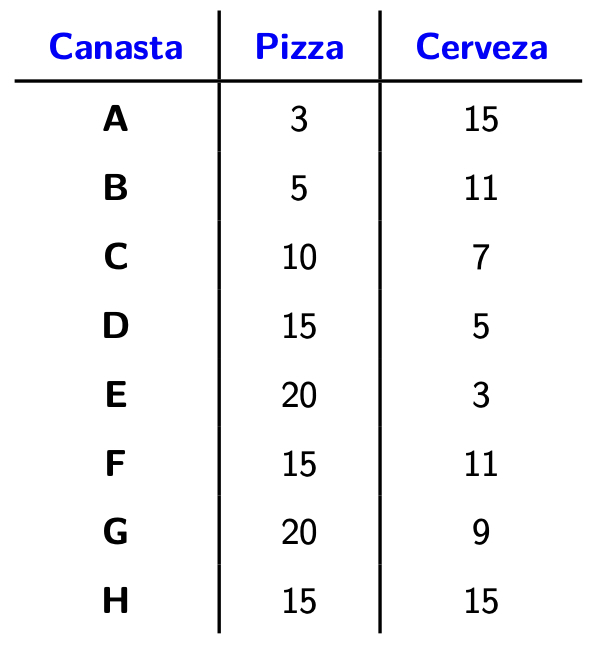
\includegraphics[width=3.5cm]{Slides Principios de Economia/Figures/tabla_canastas.jpg}};

        % Ejes
        \draw[thick,->] (0,0) -- (12,0) node[below right] {Pizza};
        \draw[thick,->] (0,0) -- (0,8.5) node[left] {Cerveza};
        
         % Etiquetas de cantidades de cerveza
        \node[left] at (0,7.5) {15};
        \node[left] at (0,5.5) {11};
        \node[left] at (0,4.5) {9};
        \node[left] at (0,3.5) {7};
        \node[left] at (0,2.5) {5};
        \node[left] at (0,1.5) {3};

        % Etiquetas de cantidades de pizza
        \node[below] at (1.5,0) {3};
        \node[below] at (2.5,0) {5};
        \node[below] at (5,0) {10};
        \node[below] at (7.5,0) {15};
        \node[below] at (10,0) {20};

        \only<2->{
        \draw[dashed] (0,7.5) -- (1.5,7.5);
        \draw[dashed] (1.5,7.5) --(1.5,0) ;
        \fill[red] (1.5,7.5) circle (2.5pt) node[above right] {A};
        }
        
        \only<3->{
        \draw[thick,->,blue] (1.5,7.5) -- (1.5,5.6);
        \draw[thick,->,blue] (1.5,5.5) -- (2.4,5.5);
        \draw[dashed] (0,5.5) -- (2.5,5.5);
        \draw[dashed] (2.5,5.5) --(2.5,0);
        \fill[black] (1.5,5.5) circle (2.5pt);
        \fill[red] (2.5,5.5) circle (2.5pt) node[above right] {B};
        \node[right,blue] at (1.4,6.5) {\scalebox{0.8}{4}};
        \node[above,blue] at (2,4.8) {\scalebox{0.8}{2}};
        }

        % Flechas indicando la TMT
        \only<4->{
        \draw[thick,->,blue] (2.5,5.5) -- (2.5,3.6);
        \draw[thick,->,blue] (2.5,3.5) -- (4.9,3.5);
        \draw[thick,->,blue] (5,3.5) -- (5,2.6);
        \draw[thick,->,blue] (5,2.5) -- (7.4,2.5);
        \draw[thick,->,blue] (7.5,2.5) -- (7.5,1.6);
        \draw[thick,->,blue] (7.5,1.5) -- (9.9,1.5);

        % Puntos clave en rojo
        \fill[black] (2.5,3.5) circle (2.5pt);
        \fill[red] (5,3.5) circle (2.5pt) node[above right] {C};
        \fill[black] (5,2.5) circle (2.5pt);
        \fill[black] (7.5,1.5) circle (2.5pt);
        \fill[red] (7.5,2.5) circle (2.5pt) node[above right] {D};
        \fill[red] (10,1.5) circle (2.5pt) node[above right] {E};


        % Etiquetas de TMT
        \node[right,blue] at (2.5,4.5) {\scalebox{0.8}{4}};
        \node[right,blue] at (4.9,3) {\scalebox{0.8}{2}};
        \node[above,blue] at (3.7,2.85) {\scalebox{0.8}{5}};
        \node[above,blue] at (6.3,1.85) {\scalebox{0.8}{5}};
        \node[above,blue] at (8.8,0.8) {\scalebox{0.8}{5}};
        
        % Líneas punteadas
        \draw[dashed] (0,3.5) -- (2.4,3.5);
        \draw[dashed] (0,2.5) --(4.9,2.5);
        \draw[dashed] (5,2.5) --(5,0);
        \draw[dashed] (0,1.5) --(7.4,1.5);
        \draw[dashed] (7.5,1.5) --(7.5,0);
        \draw[dashed] (10,1.5) --(10,0);
        }
        
         % F G y H
        \only<5->{
        \draw[dashed] (7.5,7.5) --(0,7.5);
        \draw[dashed] (7.5,7.5) --(7.5,0);

        \draw[dashed] (0,5.5) --(7.5,5.5);
        \draw[dashed] (0,4.5) --(10,4.5);
        \draw[dashed] (10,4.5) --(10,1.5);
        \fill[red] (7.5,7.5) circle (2.5pt) node[above right] {H};
        \fill[red] (7.5,5.5) circle (2.5pt) node[above right] {F};
        \fill[red] (10,4.5) circle (2.5pt) node[above right] {G};
        }

    \end{tikzpicture}
\end{center}
\end{frame}

\begin{frame}
\frametitle{Algunas nos dejan igual de feliz}
Supongamos que el estudiante revela que se encuentra indiferente entre las canastas A, B, C, D y E.

\begin{center}
    \begin{tikzpicture}[scale=0.6]

        % Ejes
        \draw[thick,->] (0,0) -- (12,0) node[below right] {Pizza};
        \draw[thick,->] (0,0) -- (0,8.5) node[left] {Cerveza};
        
         % Etiquetas de cantidades de cerveza
        \node[left] at (0,7.5) {15};
        \node[left] at (0,5.5) {11};
        \node[left] at (0,4.5) {9};
        \node[left] at (0,3.5) {7};
        \node[left] at (0,2.5) {5};
        \node[left] at (0,1.5) {3};

        % Etiquetas de cantidades de pizza
        \node[below] at (1.5,0) {3};
        \node[below] at (2.5,0) {5};
        \node[below] at (5,0) {10};
        \node[below] at (7.5,0) {15};
        \node[below] at (10,0) {20};

        % Puntos clave en rojo
        \fill[red] (1.5,7.5) circle (2.5pt) node[above right] {A};
        \fill[red] (2.5,5.5) circle (2.5pt) node[above right] {B};
        \fill[red] (5,3.5) circle (2.5pt) node[above right] {C};
        \fill[red] (7.5,2.5) circle (2.5pt) node[above right] {D};
        \fill[red] (10,1.8) circle (2.5pt) node[above right] {E};

         % F G y H
        \fill[red] (7.5,7.5) circle (2.5pt) node[above right] {H};
        \fill[red] (7.5,5.5) circle (2.5pt) node[above right] {F};
        \fill[red] (10,4.5) circle (2.5pt) node[above right] {G};
        
        % Curva de indiferencia
        \only<2->{
        \draw[thick, red] plot[smooth, tension=0.4] coordinates {(1.3,8) (1.5,7.5) (2.5,5.5) (3.5,4.5) (5,3.5) (7.5,2.5) (10,1.8) (11,1.6)};
        }
        \only<3->{
        \draw[thick, red] plot[smooth, tension=0.4] coordinates {(4.65,8) (5.1,7.5) (6.1,6.5) (7.5,5.5) (8.5,5) (10,4.5) (11,4.3)};
        }
        \only<4->{
        \draw[thick, red] plot[smooth, tension=0.4] coordinates {(7,8) (7.5,7.5) (8.5,7) (10,6.5) (11,6.3)};
        }

    \end{tikzpicture}
\end{center}
\end{frame}

\begin{frame}
\frametitle{Las curvas de indiferencia}
\begin{itemize}
    \item Todas las posibles canastas que otorgan el mismo nivel de utilidad o felicidad se encuentran sobre una misma \textbf{curva de indiferencia}. \vspace{2mm}
    \item ¿Qué nivel de felicidad nos dan esas canastas? 
    \begin{itemize}
    \item No nos interesa cuánto. Lo único relevante es si una canasta tiene una utilidad mayor a otra. 
    \item Vemos que las canastas F y G están sobre otra curva de indiferencia. Osea que nos dan otro nivel de utilidad. Lo mismo sucede con la canasta H. \vspace{1mm}
    \end{itemize} \pause
     \item La cantidad de curvas de indiferencia podemos suponer que es \textbf{infinita}. Esto nos forma un \textbf{mapa de indiferencia}, donde las que están más a la derecha y arriba brindan más utilidad.
    \end{itemize}
\end{frame}

\begin{frame}
\frametitle{Supuestos de la relación de preferencias}
    \begin{enumerate}
    \item \textcolor{blue}{Completitud}: Los consumidores pueden \textbf{comparar} y \textbf{ordenar} cualquier par de canastas de bienes.
    \item \textcolor{blue}{Monotonicidad fuerte}: Si una canasta tiene al menos una unidad más de un bien, entonces esa canasta es preferida. Esto implica que:
    \begin{itemize}
        \item Las curvas de indiferencia tienen pendiente negativa. 
        \item Las curvas de indiferencia más altas corresponden a niveles de utilidad más altos (más es mejor).
    \end{itemize}
    \item \textcolor{blue}{Transitividad}: Si un consumidor prefiere la canasta A a la B y la B a la C, entonces prefiere la canasta A a la C.
    \begin{itemize}
        \item Las curvas de indiferencia no se cruzan
    \end{itemize}


\item \textcolor{blue}{Convexidad}: Los consumidores prefieren consumir canastas de consumo \textit{balanceadas} antes que aquellas canastas que tienen mucho de un solo bien.
    \begin{itemize}
        \item Las curvas de indiferencia son convexas: se hacen más empinadas a la izquierda y más planas a la derecha 
    \end{itemize}
\end{enumerate} 
\end{frame}



\begin{frame}
\frametitle{¿Qué es la utilidad marginal decreciente?}
\begin{itemize}
    \item Nos dice cómo cambia la utilidad total cuando agregamos una unidad adicional de un bien, dejando constante la cantidad del otro bien.
    \item  Una porción de pizza adicional siempre aumenta la utilidad, pero a un ritmo cada vez menor, por eso decimos que es \textbf{decreciente}.
    \end{itemize}    
    \vspace{2mm}
\begin{center}
    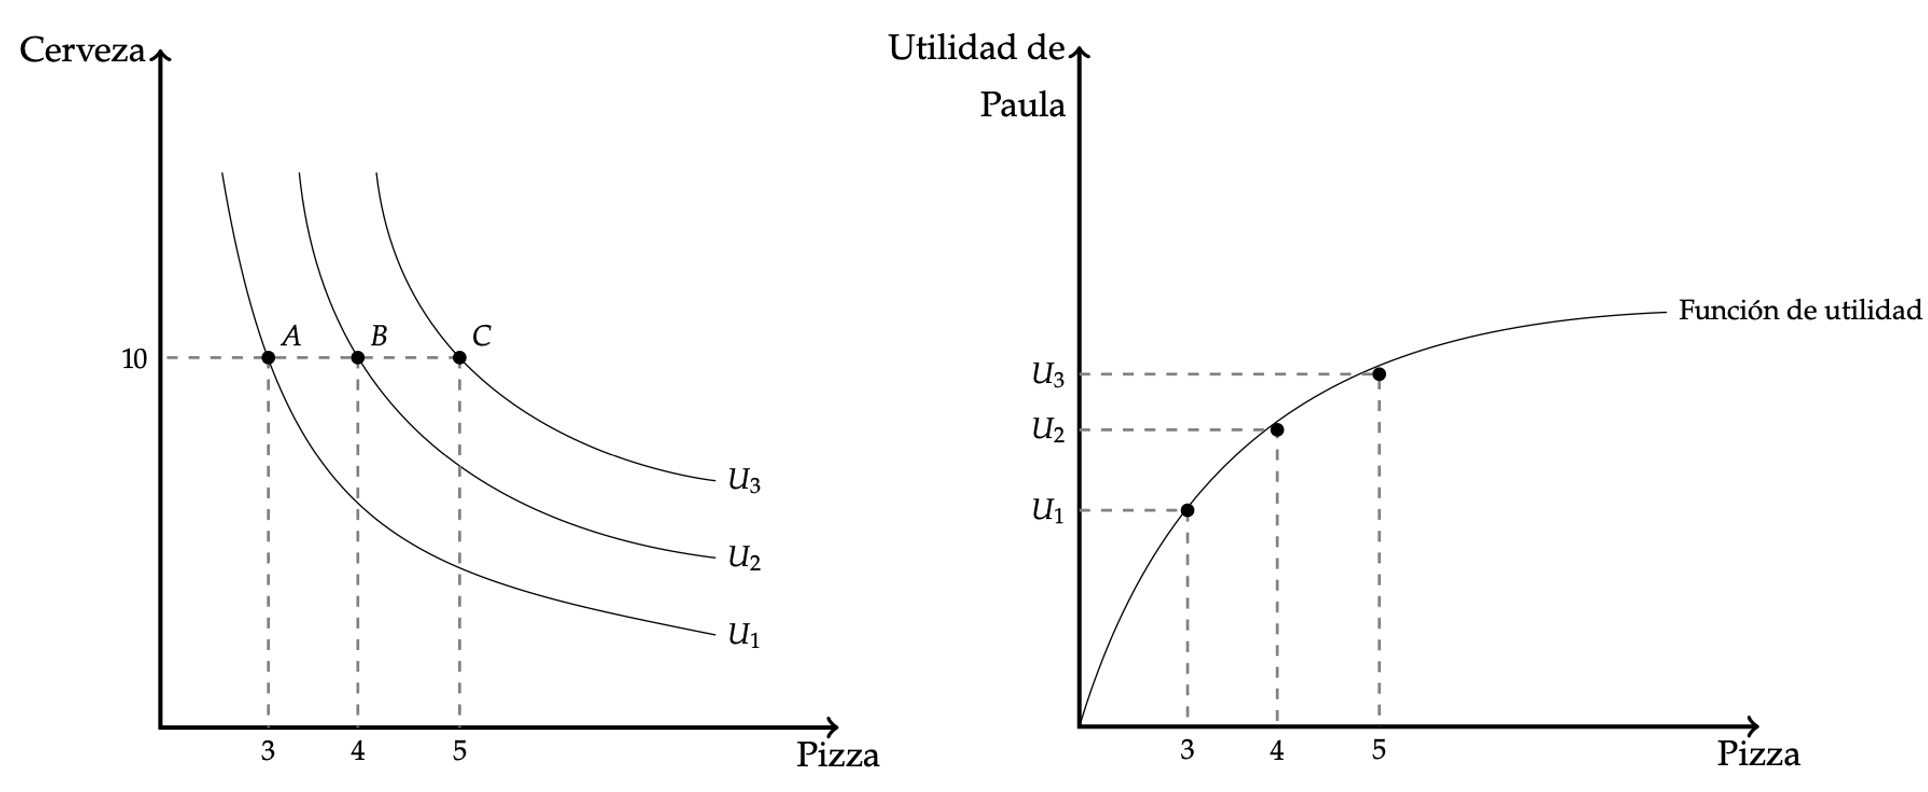
\includegraphics[scale=0.35]{Slides Principios de Economia/Figures/Umg_dec.png}
    \end{center}
\end{frame}

\begin{frame}
\frametitle{Tasa Marginal de Sustitución}

\begin{itemize}
    \item La TMS es la cantidad de unidades de un bien que el individuo está \textbf{dispuesto} a sacrificar a cambio de una unidad adicional del otro bien, de tal manera que se mantiene constante su nivel de utilidad. \vspace{2mm}
    \item Es la pendiente de las curvas de indiferencia. \pause
    \begin{center}
        $\Delta U = 0$ \\  \vspace{2mm}
        $\Delta U = UMg_x \cdot \Delta X + UMg_y \cdot \Delta Y = 0$ \\ \vspace{2mm}
        $ UMg_x \cdot \Delta X = UMg_y \cdot - \Delta Y$ \\ \vspace{2mm}
        $TMS = \frac{\Delta Y}{\Delta X} = - \frac{UMg_x}{UMg_y}$ \vspace{2mm}
    \end{center}   
    \item Intuitivamente, nos indica cuántos porrones de cerveza ($Y$) estamos dispuestos a sacrificar a cambio de consumir una porción adicional de pizza ($X$).
    \item  ¡No es constante!
\end{itemize} 
\end{frame}

\begin{frame}
\frametitle{Tasa Marginal de Sustitución}
\vspace{2mm}
\begin{itemize}
    \item  $TMS_A = -4 \Rightarrow$ estamos dispuestos a sacrificar 4 cervezas para conseguir una porción de pizza adicional.
    \item  $TMS_C = -1 \Rightarrow$ 1 cerveza por una pizza adicional.
    \item  $TMS_E = -0,5 \Rightarrow$ media cerveza por una pizza adicional (ya tenemos mucha pizza!)
\end{itemize} 
\begin{center}
    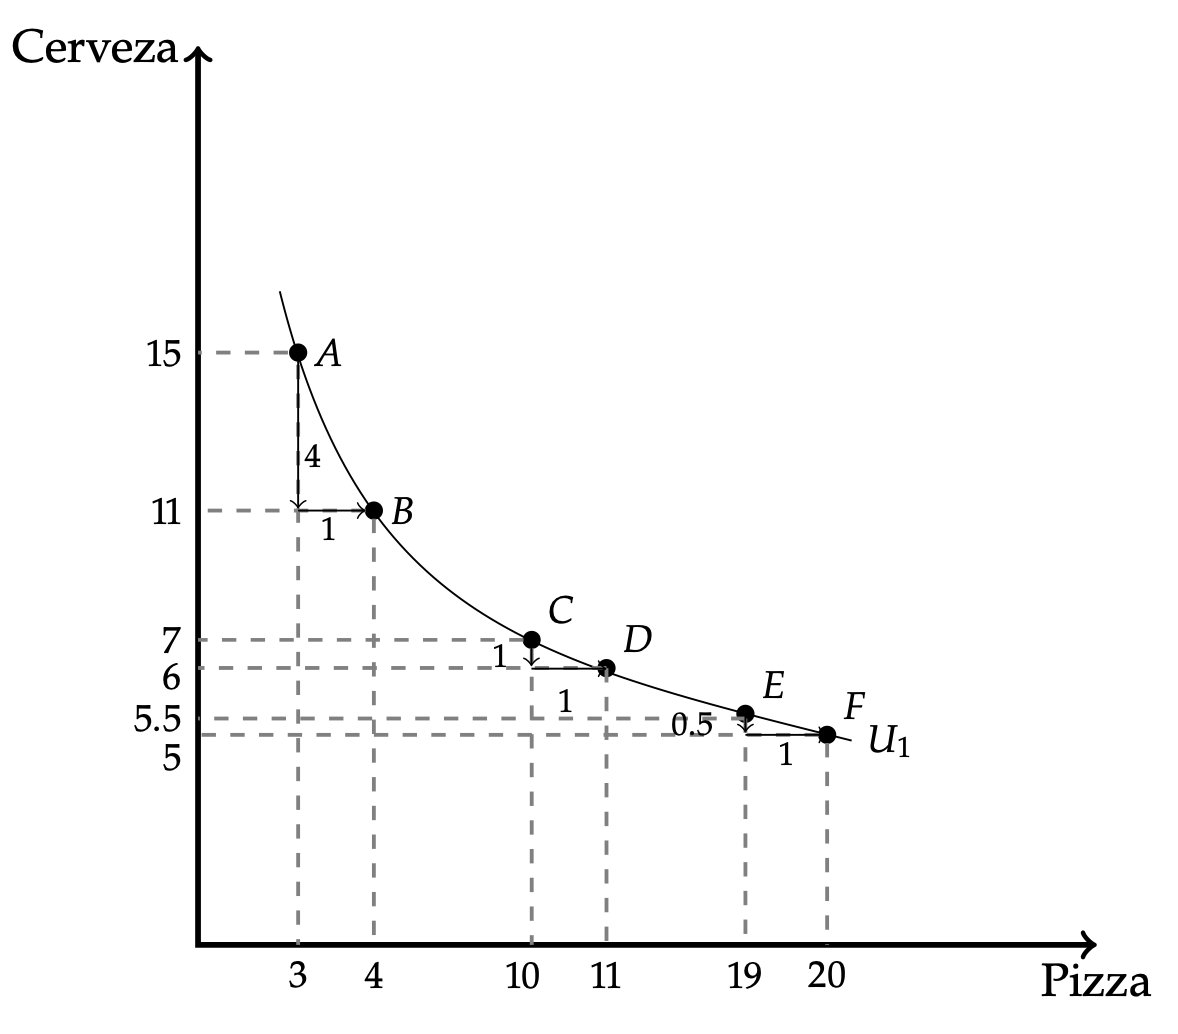
\includegraphics[scale=0.3]{Slides Principios de Economia/Figures/cambio_tms.png}
    \end{center}
\end{frame}

\begin{frame}
\frametitle{Bonus: Las curvas de indiferencias pueden tener formas diferentes}
\begin{columns}
    % Columna izquierda (texto)
    \column{0.55\textwidth}
    \begin{itemize}
        \item Bienes sustitutos perfectos
        \item Bienes complementarios perfectos
        \item Bien y mal
        \item Bien neutral
    \end{itemize}

    % Columna derecha (imagen)
    \column{0.5\textwidth}
    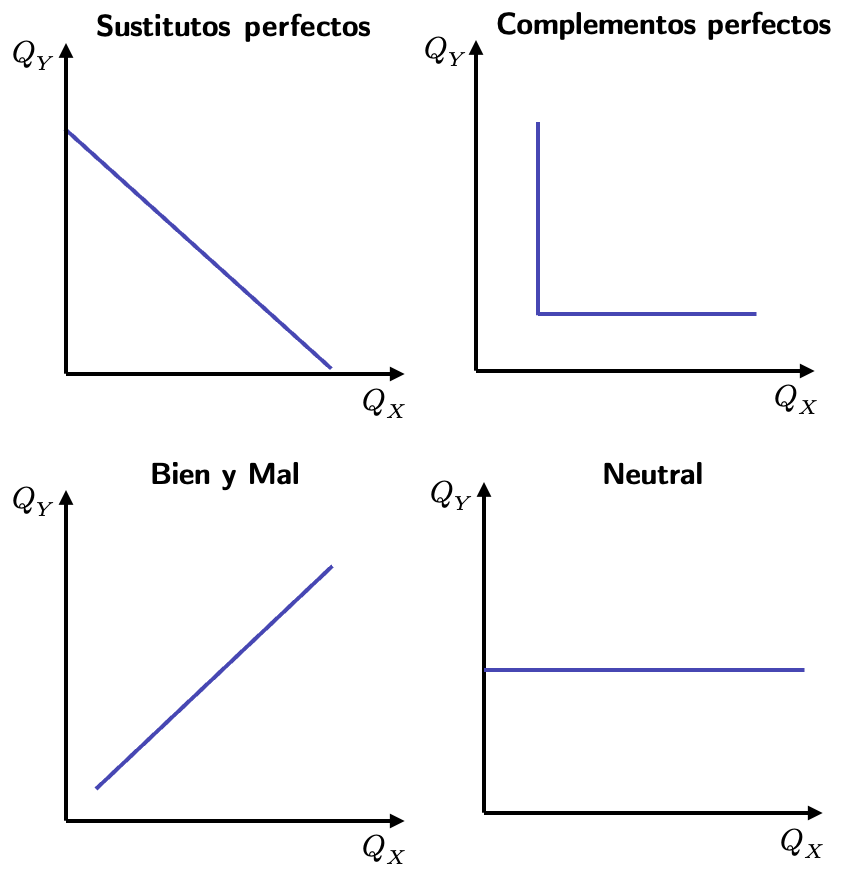
\includegraphics[scale=0.35]{Slides Principios de Economia/Figures/Magistral_03/CI_casos.png}
\end{columns}


\end{frame}

\begin{frame}
    \centering
    \begin{boxB}
    \centering \Large \textbf{TEORÍA DEL CONSUMIDOR} \\   
    \end{boxB}
     \vspace{2mm}
    \Large \textbf{La elección del individuo y la curva de demanda individual} \\
     \vspace{5mm}
    \large \textbf{Capítulo 8}
\end{frame}

\begin{frame}
\frametitle{Comportamiento del consumidor}
\begin{itemize}
    \item Se puede ver entonces a los consumidores como individuos que tienen: \vspace{-2mm}
    \begin{itemize}
        \item[1.] \textbf{Recursos limitados}. \\
        - Por lo tanto, enfrentan una restricción presupuestaria. Solo puede elegir entre las canastas de consumo alcanzables
        para él. \vspace{2mm}
        \item[2.] Ciertas \textbf{preferencias} sobre diferentes productos. Para elegir la canasta que más le gusta, debe tener en cuenta
        sus preferencias. \\ \vspace{2mm}
    \end{itemize}
    
    \item También hacemos un supuesto adicional: \vspace{2mm}
    \begin{itemize}
    \item Los individuos son \textbf{racionales}: toman la mejor decisión posible dada la información.
    \end{itemize}
\end{itemize} 
\end{frame}

\begin{frame}
\frametitle{Volviendo al problema del estudiante:}
\begin{center}
    \begin{tikzpicture}[scale=1.2]

        \node at (3,3) {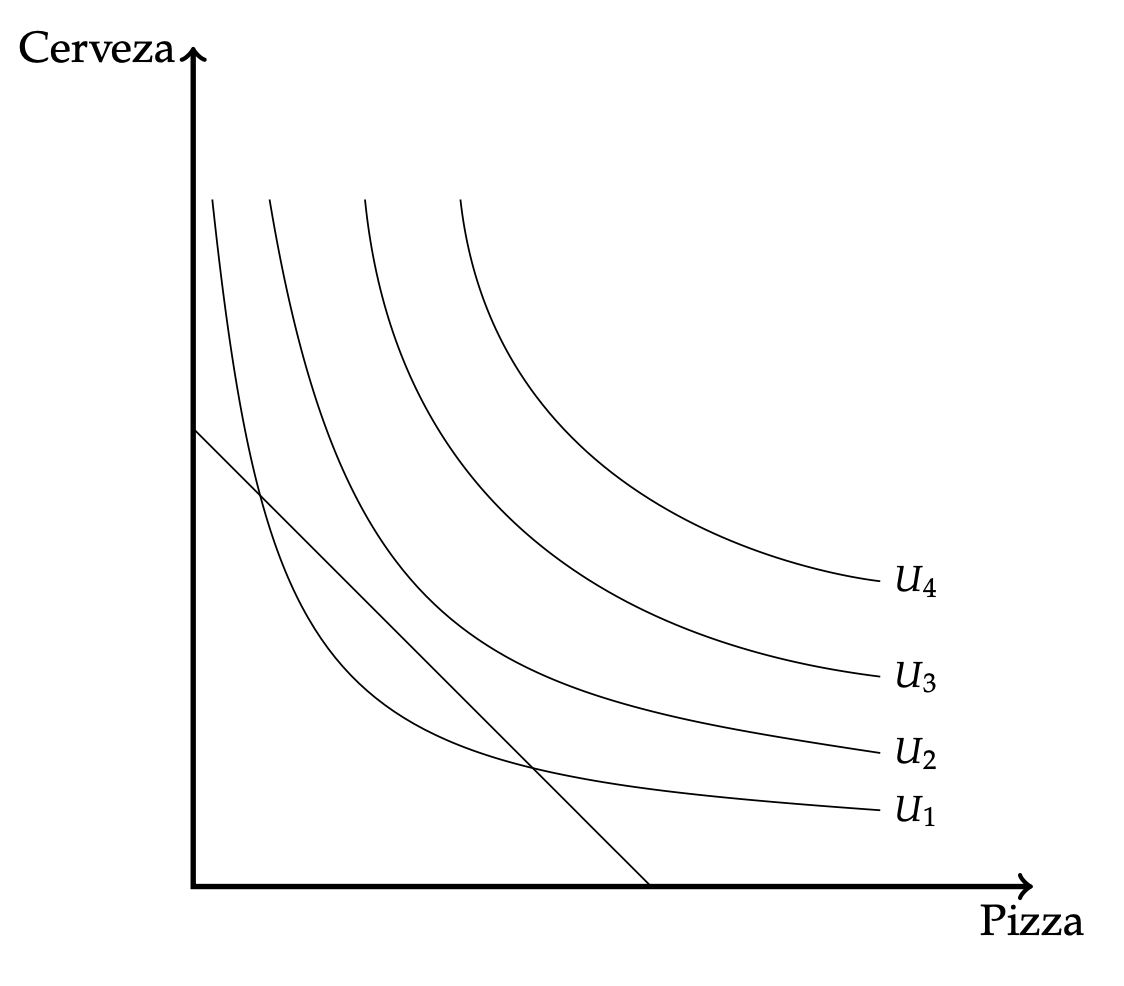
\includegraphics[width=8.5cm]{Slides Principios de Economia/Figures/problema_consumidor.png}};
        \node[right] at (-1.8,2.5) {\textbf{Restricción }};
        \node[right] at (-1.8,2) {\textbf{presupuestaria}};
        \draw[->] (0.5,2) -- (2,2);
        \node[above] at (5,3.5) {\textbf{Curvas de indiferencia}};
        \draw[->] (5,3.4) -- (4.5,3);

    \end{tikzpicture}
\end{center}
\end{frame}

\begin{frame}
\frametitle{Finalmente, ¿cómo decide el consumidor?}
\begin{itemize}
    \item Una idea central en economía es que las personas buscan maximizar su felicidad. \vspace{2mm}
    \begin{itemize}
    \item En la jerga se dice que los individuos intentan ``maximizar su utilidad''. \vspace{2mm}
    \item Pero no nos olvidemos que los individuos enfrentan una restricción presupuestaria. \vspace{2mm}
    \end{itemize} 
    \item Entonces, la pregunta central es: ¿cuál es la mayor utilidad que se puede alcanzar dada la restricción presupuestaria? \vspace{2mm}
    \begin{itemize}
    \item Nos estamos preguntando por la canasta situada en la curva de indiferencia más alta que, al mismo tiempo, sea una de las canastas factibles. 
    \vspace{2mm}
    \end{itemize} 
    \begin{boxB}
    \centering La elección del individuo se basa en maximizar su utilidad sujeto a la restricción presupuestaria
    \end{boxB}
    \end{itemize}
\end{frame}

\begin{frame}
\frametitle{Equilibrio}
\begin{center}
    \begin{tikzpicture}[scale=1.2]
        \node at (3,3) {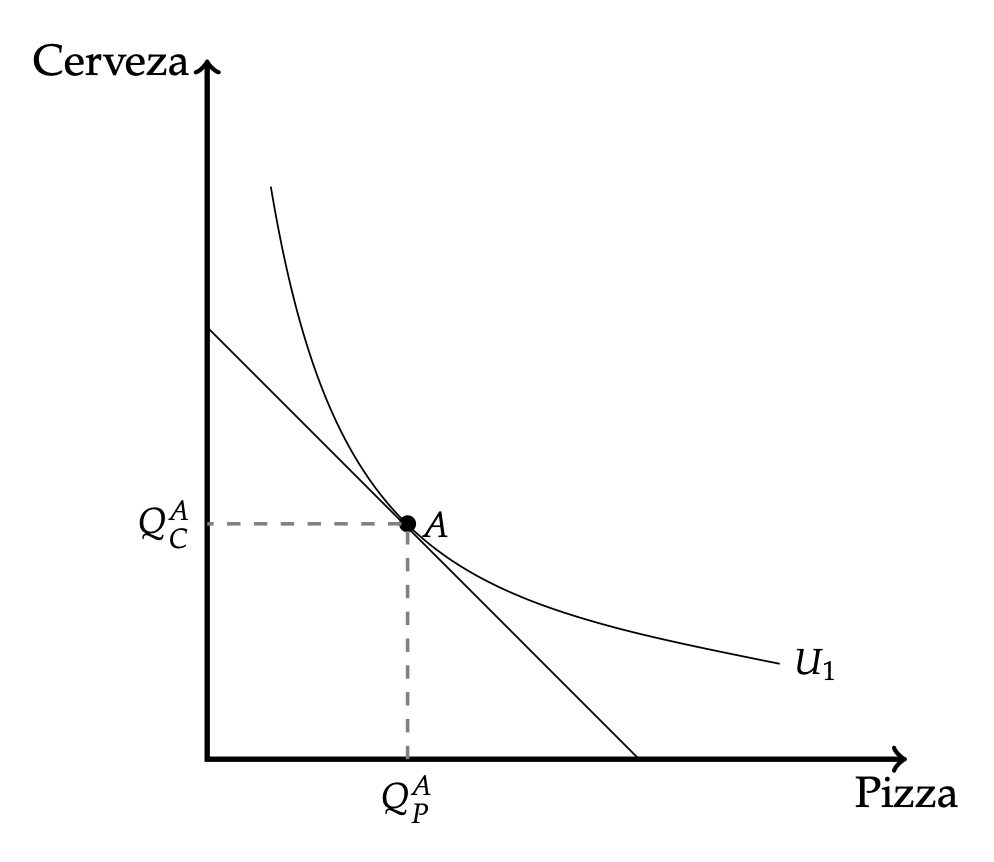
\includegraphics[width=8.5cm]{Slides Principios de Economia/Figures/equilibrio.png}};
        \node[above] at (3.5,3) {\textbf{Equilibrio}};
        \draw[->] (3,3) -- (2.5,2.5);
    \end{tikzpicture}
\end{center}
\end{frame}

\begin{frame}{Equilibrio}
    \begin{itemize}
    \item Recordemos...
    \begin{itemize}
    \footnotesize
    \item La TMS es la pendiente de la curva de indiferencia y representa la cantidad de bien Y que el consumidor está dispuesto a sacrificar por una unidad adicional del bien X, manteniendo la utilidad constante.
     \[TMS = - \frac{UMg_x}{UMg_y}\]
     \item La TMT es la pendiente de la restricción presupuestaria y muestra la relación a la cual el mercado le permite al consumidor cambiar un bien por otro
    \[TMT = - \frac{P_x}{P_y}\]
    \end{itemize}
     \normalsize
        \item La \textbf{canasta óptima} es aquella en la que la $TMS = TMT$. 
    \begin{itemize}
    \item Esto significa que lo que el consumidor está dispuesto a sacrificar del bien Y por una unidad adicional de bien X es igual a lo que el mercado le pide por esa unidad adicional de bien X.
    \item Es el punto de tangencia entre la restricción presupuestaria y una curva de indiferencia
    \end{itemize}
    \end{itemize}
\end{frame}

\begin{frame}
\frametitle{¿Por qué B no es el punto donde se maximiza la utilidad?}
\begin{center}
    \begin{tikzpicture}[scale=1.2]
        \node at (3,3) {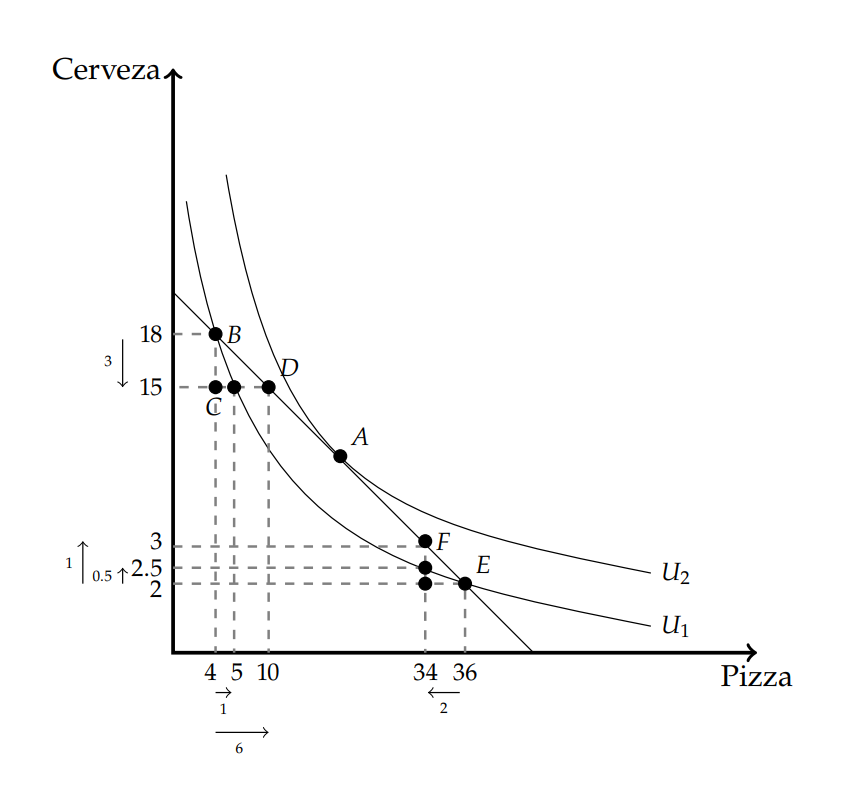
\includegraphics[width=8.5cm]{Slides Principios de Economia/Figures/C8.3.png}};
        \only<2->{
        \node[above] at (6.5,5) {\textbf{$TMS_B = -3$}};
        \node[above] at (6.5,4.5) {\small En B estamos \textbf{dispuestos} a};
        \node[above] at (6.5,4.2) {\small sacrificar 3 cervezas por 1 pizza...};
        }
        \only<3->{
        \node[above] at (6.5,3.4) {\small pero, \textbf{dados los precios}, solo};
        \node[above] at (6.5,3.1) {\small deberíamos resignar 1/2 cerveza!};
        \node[above] at (6.5,2.6) {\textbf{$TMT_B = -1/2$}};
        }
    \end{tikzpicture}
\end{center}
\end{frame}

\begin{frame}
\frametitle{Respuesta a shocks (ceteris paribus)}
\begin{itemize}
    \item Queremos ver qué sucede con la decisión del individuo cuando se producen distintos shocks. \vspace{2mm}
    \item Vamos a pensar este shock siguiendo este orden lógico:
    \begin{itemize}
        \item Partiremos de un equilibrio.
        \item Propondremos un shock sobre una variable, pero el resto de las variables se mantendrán constantes (\textit{ceteris paribus}).
        \item Discutiremos cómo impacta el shock en la restricción presupuestaria.      
        \item Discutiremos cómo impacta el cambio en la restricción a la decisión de consumo del individuo
    \end{itemize}
\end{itemize} 
\end{frame}

\begin{frame}
\frametitle{Partimos de un equilibrio:}
\begin{center}
\begin{figure}[H]
\renewcommand{\figurename}{Figure}
\begin{center}
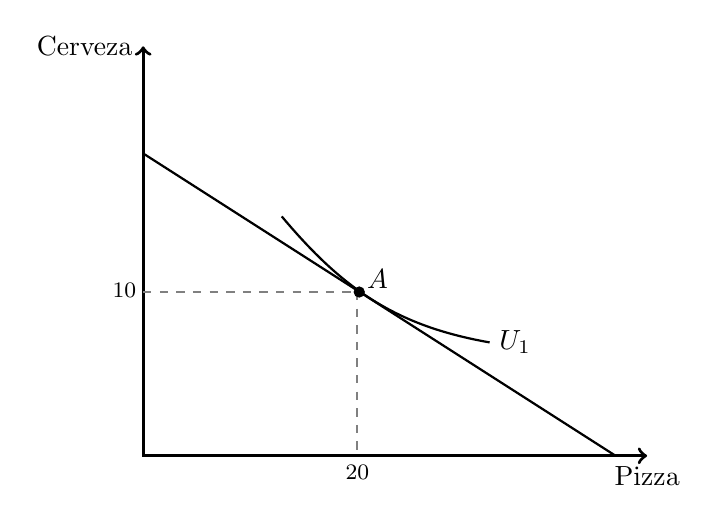
\begin{tikzpicture}[scale=0.8]
\draw[very thick,<->] (0,6.5) node[left]{Cerveza}--(0,0)--(8,0) node[below]{Pizza};
\draw [thick] (2.2,3.8) to [out=310,in=170] (5.5,1.8);
\node [right] at (5.5,1.8) {$U_1$};
\draw[thick, dashed,gray](0,2.6)--(3.4,2.6);
\node[below] at (-0.3,2.9) {\footnotesize 10};
\node[below] at (3.4,0) {\footnotesize 20};
\draw [thick] (0,4.8) -- (7.5,0);
\draw[thick, dashed,gray](3.4,2.6)--(3.4,0);
\node [right] at (3.4,2.8) {$A$};
\draw[fill] (3.43,2.6) circle [radius =0.08];
\end{tikzpicture}
\end{center}
\end{figure}
\end{center}
\end{frame}

\begin{frame}
\frametitle{Cuando hay un shock en el ingreso}
\begin{itemize}
    \item Ceteris paribus: manteniendo todo lo demás constante.
    \item La restricción presupuestaria se desplaza de manera \textbf{paralela} hacia la derecha (con aumento de ingreso) o hacia la izquierda (con disminución de ingreso).
    \item El consumidor va a tener un conjunto factible diferente.
    \item El cambio en el ingreso no altera los precios relativos.
    \item Habrá una nueva canasta óptima para el consumidor, que dependerá de las preferencias del individuo por los bienes en cuestión, es decir, de la forma que presenten las curvas de indiferencia. 
\end{itemize}
\end{frame}

\begin{frame}{Aumentan las cantidades demandadas (bienes normales)}
    \centering
    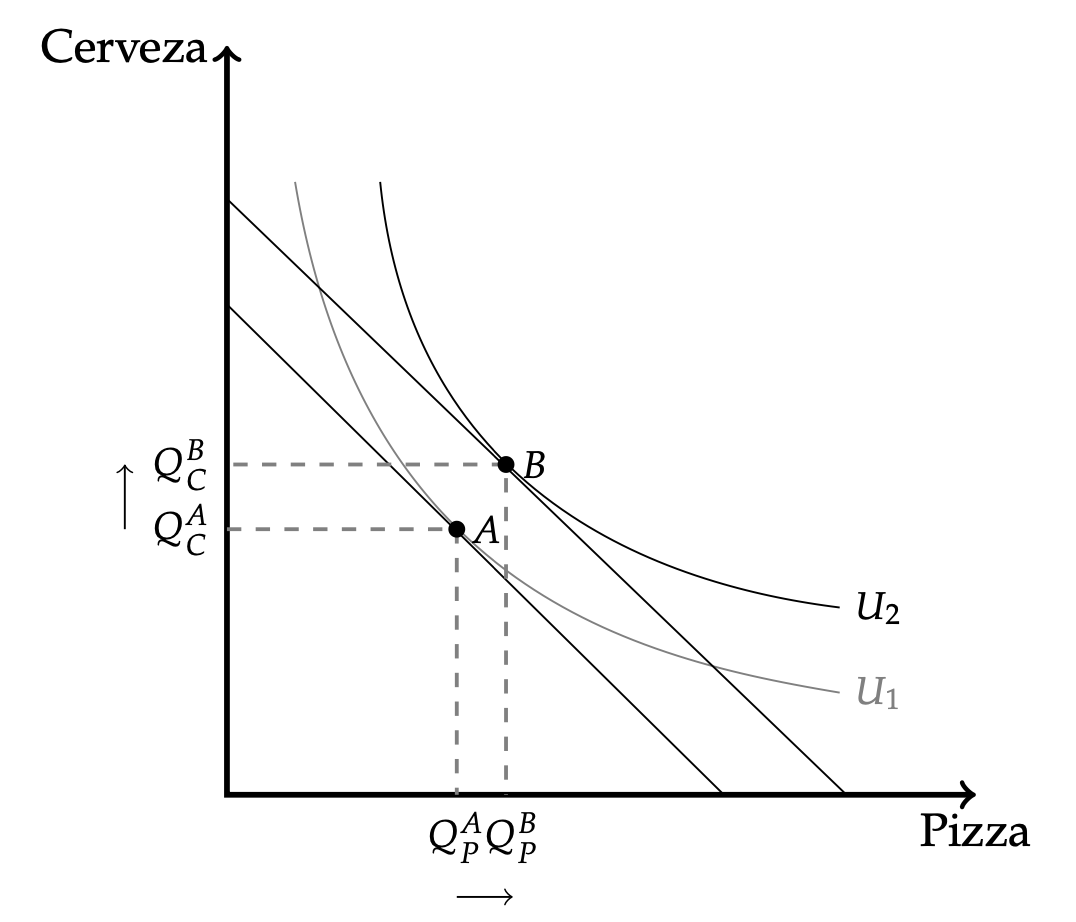
\includegraphics[scale=0.45]{../Figures/C.8.4.png}
\end{frame}

\begin{frame}{Disminuyen las cantidades demandadas (bienes inferiores)}
    \centering
    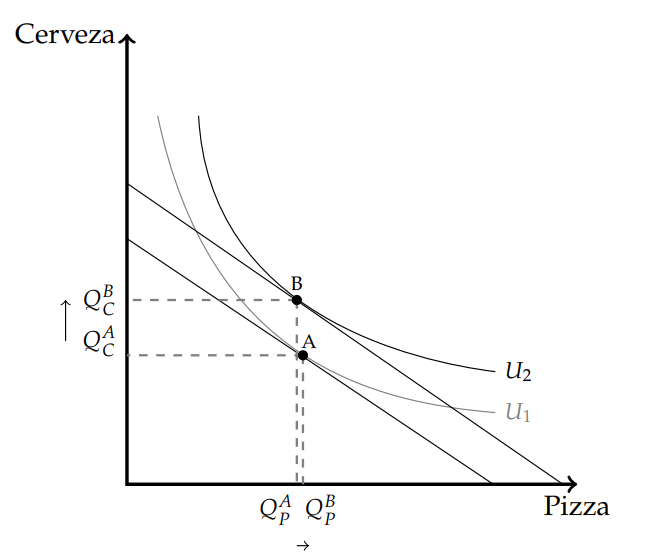
\includegraphics[scale=0.45]{../Figures/C.8.5.png}
\end{frame}

\begin{frame}{Se mantienen constantes las cantidades demandadas (bienes neutrales)}
    \centering
    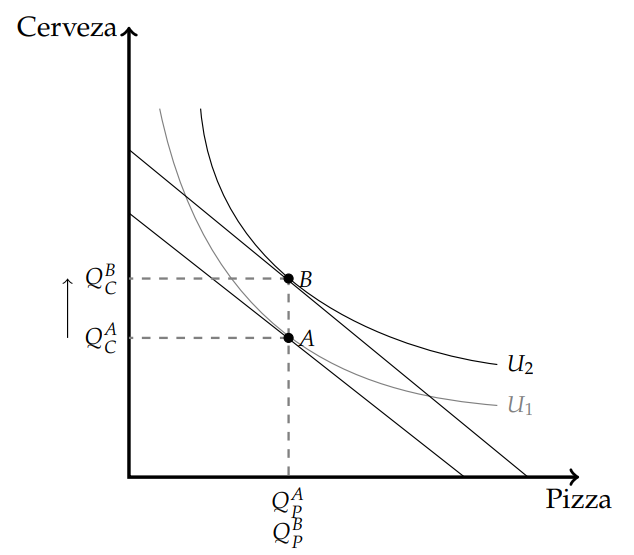
\includegraphics[scale=0.45]{../Figures/C.8.6.png}
\end{frame}

\begin{frame}
\frametitle{Cuando hay un shock en el precio de un bien}
\begin{itemize}
    \item Ceteris paribus: manteniendo todo lo demás constante.
    \item La restricción presupuestaria \textbf{pivotea} sobre el bien que no cambia el precio, reduciendo (aumentando) la cantidad máxima del bien afectado por el aumento (disminución) del precio.  
    \item El consumidor va a tener menos (más) canastas disponibles porque su conjunto factible se ha reducido (expandido).
    \item El cambio en el precio de un bien también altera los precios relativos. 
    \item Habrá una nueva canasta óptima para el consumidor.
\end{itemize}
\end{frame}

\begin{frame}
\frametitle{1. Partimos del equilibrio A y aumenta el precio de la pizza}
\begin{center}
\begin{figure}[H]
\renewcommand{\figurename}{Figure}
\begin{center}
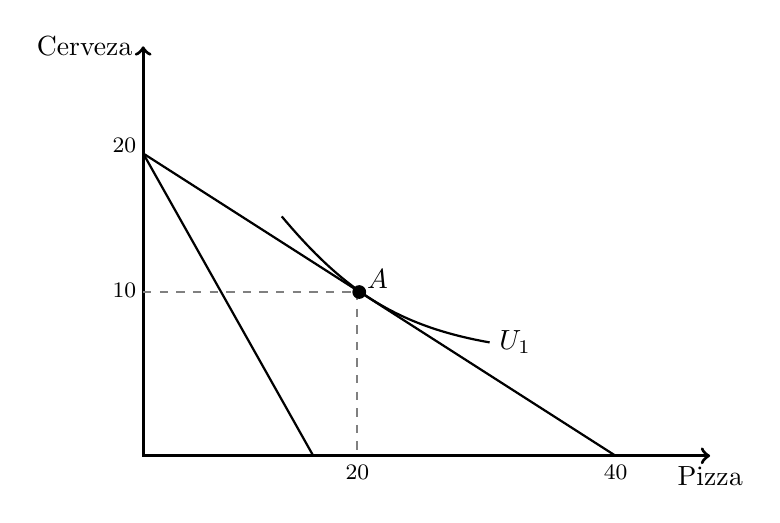
\begin{tikzpicture}[scale=0.8]
\draw[very thick,<->] (0,6.5) node[left]{Cerveza}--(0,0)--(9,0) node[below]{Pizza};
\draw [thick] (2.2,3.8) to [out=310,in=170] (5.5,1.8);
\node [right] at (5.5,1.8) {$U_1$};
\node[below] at (3.4,0) {\footnotesize 20};
\node[below] at (7.5,0) {\footnotesize 40};
\draw [thick] (0,4.8) -- (7.5,0);
\draw [thick] (0,4.8) -- (2.7,0);
\draw[thick, dashed,gray](0,2.6)--(3.4,2.6);
\node[below] at (-0.3,2.9) {\footnotesize 10};
\node[below] at (-0.3,5.2) {\footnotesize 20};
\draw[thick, dashed,gray](3.4,2.6)--(3.4,0);
\node [right] at (3.4,2.8) {$A$};
\draw[fill] (3.43,2.6) circle [radius =0.1];
\end{tikzpicture}
\end{center}
\end{figure}
\end{center}
\end{frame}

\begin{frame}
\frametitle{2. La nueva canasta óptima es B}
\begin{center}
\begin{figure}[H]
\renewcommand{\figurename}{Figure}
\begin{center}
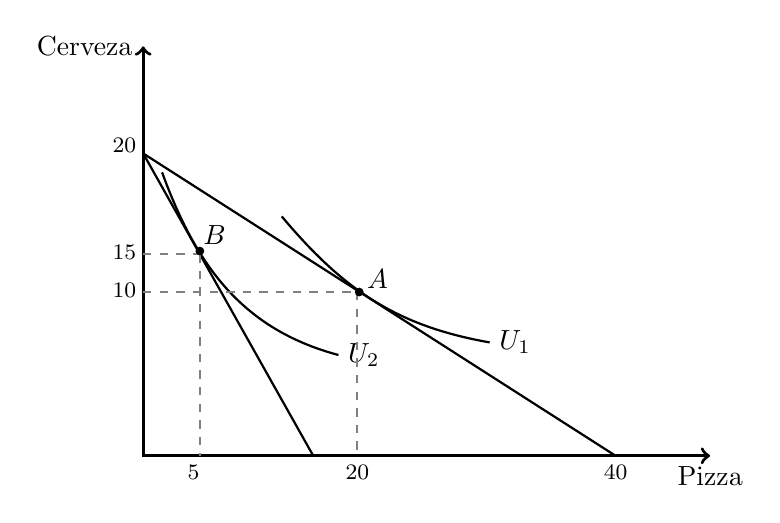
\begin{tikzpicture}[scale=0.8]
\draw[very thick,<->] (0,6.5) node[left]{Cerveza}--(0,0)--(9,0) node[below]{Pizza};
\draw [thick] (2.2,3.8) to [out=310,in=170] (5.5,1.8);
\node [right] at (5.5,1.8) {$U_1$};
\draw [thick] (0.3,4.5) to [out=290,in=165] (3.1,1.6);
\node [right] at (3.1,1.6) {$U_2$};
\node[below] at (3.4,0) {\footnotesize 20};
\node[below] at (7.5,0) {\footnotesize 40};
\node[below] at (0.8,0) {\footnotesize 5};
\draw [thick] (0,4.8) -- (7.5,0);
\draw [thick] (0,4.8) -- (2.7,0);
\draw[thick, dashed,gray](0.9,3.2)--(0.9,0);
\draw[thick, dashed,gray](0,3.2)--(0.9,3.2);
\node[below] at (-0.3,3.5) {\footnotesize 15};
\draw[thick, dashed,gray](0,2.6)--(3.4,2.6);
\node[below] at (-0.3,2.9) {\footnotesize 10};
\node[below] at (-0.3,5.2) {\footnotesize 20};
\draw[thick, dashed,gray](3.4,2.6)--(3.4,0);
\node [right] at (0.8,3.5) {$B$};
\draw[fill] (0.9,3.25) circle [radius =0.06];
\node [right] at (3.4,2.8) {$A$};
\draw[fill] (3.43,2.6) circle [radius =0.06];
\end{tikzpicture}
\end{center}
\end{figure}
\end{center}
\end{frame}

\begin{frame}
\frametitle{3. El efecto total de un aumento en el precio de la pizza} 
\begin{center}
\begin{figure}[H]
\renewcommand{\figurename}{Figure}
\begin{center}
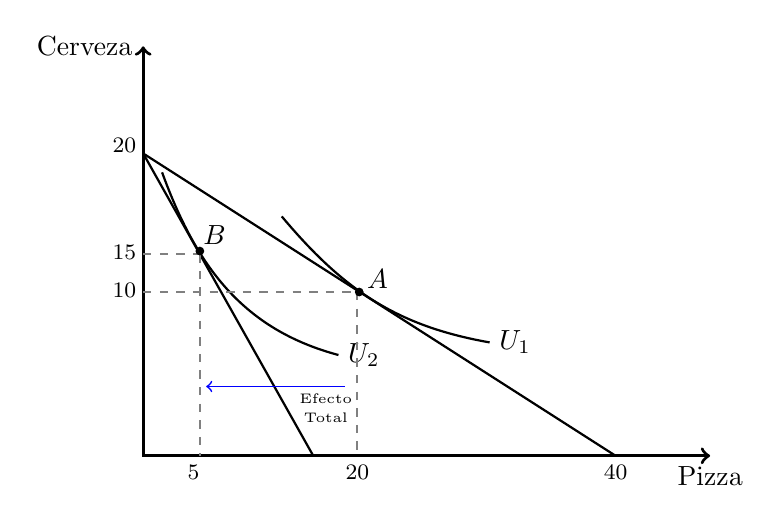
\begin{tikzpicture}[scale=0.8]
\draw[very thick,<->] (0,6.5) node[left]{Cerveza}--(0,0)--(9,0) node[below]{Pizza};
\draw [thick] (2.2,3.8) to [out=310,in=170] (5.5,1.8);
\node [right] at (5.5,1.8) {$U_1$};
\draw [thick] (0.3,4.5) to [out=290,in=165] (3.1,1.6);
\node [right] at (3.1,1.6) {$U_2$};
\node[below] at (3.4,0) {\footnotesize 20};
\node[below] at (7.5,0) {\footnotesize 40};
\node[below] at (0.8,0) {\footnotesize 5};
\draw [thick] (0,4.8) -- (7.5,0);
\draw [thick] (0,4.8) -- (2.7,0);
\draw[thick, dashed,gray](0.9,3.2)--(0.9,0);
\draw[thick, dashed,gray](3.4,2.6)--(3.4,0);
\draw[semithick, blue, <-] (1,1.1)--(3.2,1.1);
\draw[thick, dashed,gray](0,3.2)--(0.9,3.2);
\node[below] at (-0.3,3.5) {\footnotesize 15};
\draw[thick, dashed,gray](0,2.6)--(3.4,2.6);
\node[below] at (-0.3,2.9) {\footnotesize 10};
\node[below] at (-0.3,5.2) {\footnotesize 20};
\node[] at (2.9,0.9){\tiny Efecto};
\node[] at (2.9,0.6){\tiny Total};
\node [right] at (0.8,3.5) {$B$};
\draw[fill] (0.9,3.25) circle [radius =0.06];
\node [right] at (3.4,2.8) {$A$};
\draw[fill] (3.43,2.6) circle [radius =0.06];
\end{tikzpicture}
\end{center}
\end{figure}
\end{center}
\end{frame}

\begin{frame}
\frametitle{El efecto ingreso y el efecto sustitución}
\begin{itemize}
    \item Un aumento en el precio de la pizza produce dos efectos:
    \begin{itemize}
        \item Disminuye el poder de compra, porque el consumidor tiene menor poder adquisitivo.
        \item Aumenta el costo de oportunidad de la pizza, porque el precio relativo de la pizza ha aumentado (ahora es una cerveza entera!).
    \end{itemize}
    \item \textbf{Efecto ingreso}: 
     \begin{itemize}
     \item Efecto en la cantidad demandada debido al cambio en el poder adquisitivo. Es decir, es el efecto por cambios en el ingreso, dejando los precios constantes.
     \item Gráficamente, "es como2 si la restricción se desplazara hacia adentro.
    \end{itemize}
     
    \item \textbf{Efecto sustitución}:
    \begin{itemize}
     \item Efecto en la cantidad demandada debido al cambio en el costo de oportunidad. Es decir, es el efecto por cambios en los precios relativos, dejando el nivel de utilidad constante.
     \item Gráficamente, la restricción pivotea porque cambia su pendiente (TMT).
    \end{itemize}
\end{itemize} 
\end{frame}

\begin{frame}
\frametitle{Si le damos menos dinero para que esté sobre $U_2$, ¿elige B?}
\begin{center}
\begin{figure}[H]
\renewcommand{\figurename}{Figure}
\begin{center}
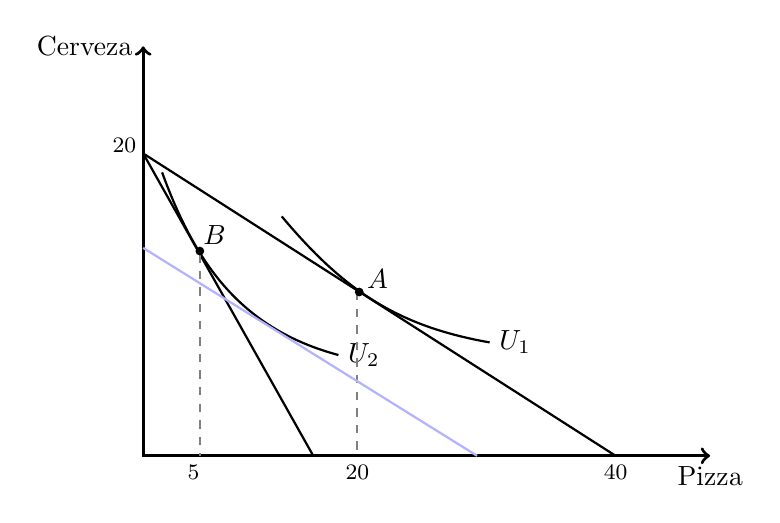
\begin{tikzpicture}[scale=0.8]
\draw[very thick,<->] (0,6.5) node[left]{Cerveza}--(0,0)--(9,0) node[below]{Pizza};
\draw [thick] (2.2,3.8) to [out=310,in=170] (5.5,1.8);
\node [right] at (5.5,1.8) {$U_1$};
\draw [thick] (0.3,4.5) to [out=290,in=165] (3.1,1.6);
\node [right] at (3.1,1.6) {$U_2$};
\node[below] at (3.4,0) {\footnotesize 20};
\node[below] at (7.5,0) {\footnotesize 40};
\node[below] at (0.8,0) {\footnotesize 5};
\node[below] at (-0.3,5.2) {\footnotesize 20};
\draw [thick] (0,4.8) -- (7.5,0);
\draw [thick] (0,4.8) -- (2.7,0);
\draw[thick, dashed,gray](0.9,3.2)--(0.9,0);
\draw[thick, dashed,gray](3.4,2.6)--(3.4,0);
\draw [thick, blue!30] (0,3.3) -- (5.3,0);
\node [right] at (0.8,3.5) {$B$};
\draw[fill] (0.9,3.25) circle [radius =0.06];
\node [right] at (3.4,2.8) {$A$};
\draw[fill] (3.43,2.6) circle [radius =0.06];
\end{tikzpicture}
\end{center}
\end{figure}
\end{center}
\end{frame}

\begin{frame}
\frametitle{No, ¡elige C!}
\begin{center}
\begin{figure}[H]
\renewcommand{\figurename}{Figure}
\begin{center}
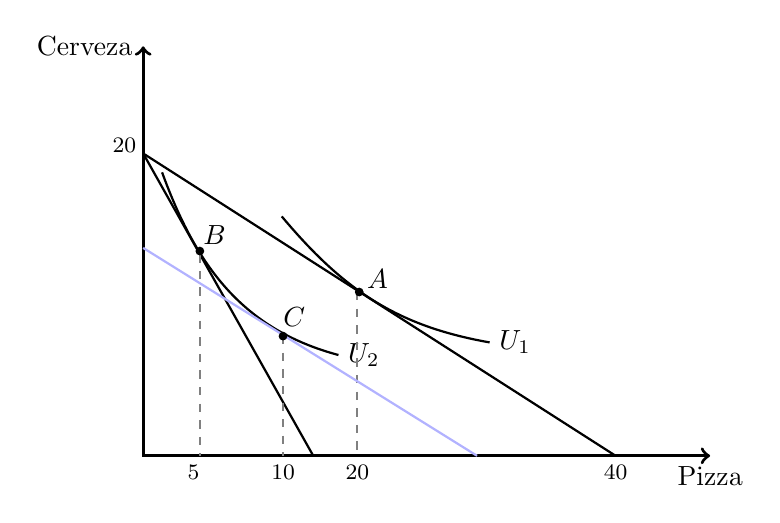
\begin{tikzpicture}[scale=0.8]
\draw[very thick,<->] (0,6.5) node[left]{Cerveza}--(0,0)--(9,0) node[below]{Pizza};
\draw [thick] (2.2,3.8) to [out=310,in=170] (5.5,1.8);
\node [right] at (5.5,1.8) {$U_1$};
\draw [thick] (0.3,4.5) to [out=290,in=165] (3.1,1.6);
\node [right] at (3.1,1.6) {$U_2$};
\node[below] at (3.4,0) {\footnotesize 20};
\node[below] at (7.5,0) {\footnotesize 40};
\node[below] at (2.22,0) {\footnotesize 10};
\node[below] at (0.8,0) {\footnotesize 5};
\node[below] at (-0.3,5.2) {\footnotesize 20};
\draw [thick] (0,4.8) -- (7.5,0);
\draw [thick] (0,4.8) -- (2.7,0);
\draw[thick, dashed,gray](0.9,3.2)--(0.9,0);
\draw[thick, dashed,gray](3.4,2.6)--(3.4,0);
\draw[thick, dashed,gray](2.22,1.9)--(2.22,0);
\draw [thick, blue!30] (0,3.3) -- (5.3,0);
\node [above] at (2.4,1.9) {$C$};
\draw[fill] (2.22,1.9) circle [radius =0.06];
\node [right] at (0.8,3.5) {$B$};
\draw[fill] (0.9,3.25) circle [radius =0.06];
\node [right] at (3.4,2.8) {$A$};
\draw[fill] (3.43,2.6) circle [radius =0.06];
\end{tikzpicture}
\end{center}
\end{figure}
\end{center}
\end{frame}

\begin{frame}
\frametitle{El efecto ingreso}
\begin{center}
\begin{figure}[H]
\renewcommand{\figurename}{Figure}
\begin{center}
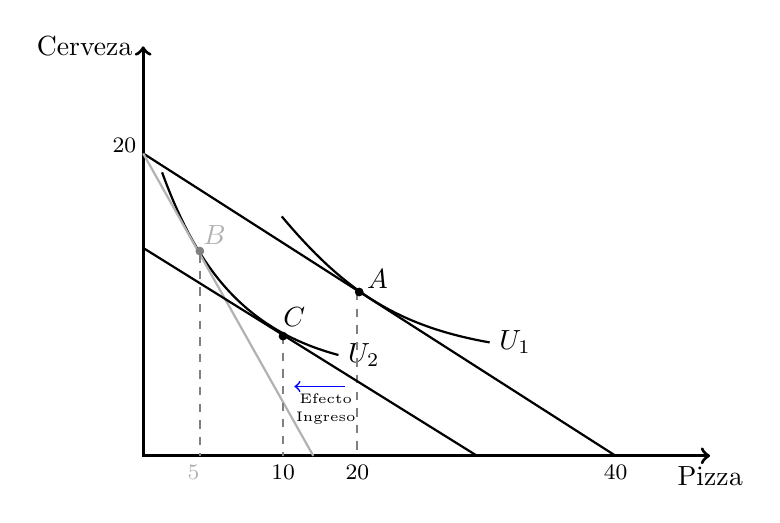
\begin{tikzpicture}[scale=0.8]
\draw[very thick,<->] (0,6.5) node[left]{Cerveza}--(0,0)--(9,0) node[below]{Pizza};
\draw [thick] (2.2,3.8) to [out=310,in=170] (5.5,1.8);
\node [right] at (5.5,1.8) {$U_1$};
\draw [thick] (0.3,4.5) to [out=290,in=165] (3.1,1.6);
\node [right] at (3.1,1.6) {$U_2$};
\node[below] at (3.4,0) {\footnotesize 20};
\node[below] at (7.5,0) {\footnotesize 40};
\node[below] at (-0.3,5.2) {\footnotesize 20};
\node[below] at (2.22,0) {\footnotesize 10};
\node[below,gray!60] at (0.8,0) {\footnotesize 5};
\draw [thick] (0,4.8) -- (7.5,0);
\draw [thick,gray!60] (0,4.8) -- (2.7,0);
\draw[thick, dashed,gray](0.9,3.2)--(0.9,0);
\draw[thick, dashed,gray](3.4,2.6)--(3.4,0);
\draw[thick, dashed,gray](2.22,1.9)--(2.22,0);
\draw [thick] (0,3.3) -- (5.3,0);
\draw[semithick, blue, <-] (2.4,1.1)--(3.2,1.1);
\node[] at (2.9,0.9){\tiny Efecto};
\node[] at (2.9,0.6){\tiny Ingreso};
\node [above] at (2.4,1.9) {$C$};
\draw[fill] (2.22,1.9) circle [radius =0.06];
\node [right,gray!60] at (0.8,3.5) {$B$};
\draw[fill,gray] (0.9,3.25) circle [radius =0.06];
\node [right] at (3.4,2.8) {$A$};
\draw[fill] (3.43,2.6) circle [radius =0.06];
\end{tikzpicture}
\end{center}
\end{figure}
\end{center}
\end{frame}



\begin{frame}
\frametitle{El efecto sustitución}
\begin{center}
\begin{figure}[H]
\renewcommand{\figurename}{Figure}
\begin{center}
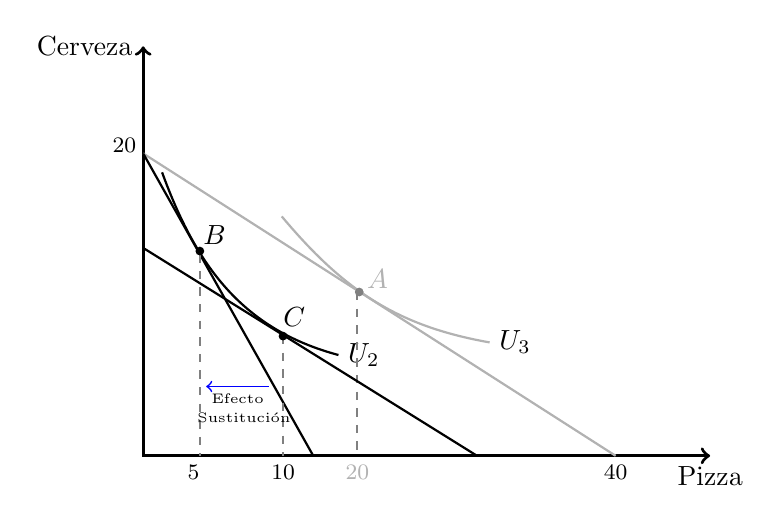
\begin{tikzpicture}[scale=0.8]
\draw[very thick,<->] (0,6.5) node[left]{Cerveza}--(0,0)--(9,0) node[below]{Pizza};
\draw [thick,gray!60] (2.2,3.8) to [out=310,in=170] (5.5,1.8);
\node [right] at (5.5,1.8) {$U_3$};
\draw [thick] (0.3,4.5) to [out=290,in=165] (3.1,1.6);
\node [right] at (3.1,1.6) {$U_2$};
\node[below,gray!60] at (3.4,0) {\footnotesize 20};
\node[below] at (7.5,0) {\footnotesize 40};
\node[below] at (-0.3,5.2) {\footnotesize 20};
\node[below] at (2.22,0) {\footnotesize 10};
\node[below] at (0.8,0) {\footnotesize 5};
\draw [thick,gray!60] (0,4.8) -- (7.5,0);
\draw [thick] (0,4.8) -- (2.7,0);
\draw[thick, dashed,gray](0.9,3.2)--(0.9,0);
\draw[thick, dashed,gray](3.4,2.6)--(3.4,0);
\draw[thick, dashed,gray](2.22,1.9)--(2.22,0);
\draw [thick] (0,3.3) -- (5.3,0);
\draw[semithick, blue, <-] (1,1.1)--(2,1.1);
\node[] at (1.5,0.9){\tiny Efecto};
\node[] at (1.6,0.6){\tiny Sustitución};
\node [above] at (2.4,1.9) {$C$};
\draw[fill] (2.22,1.9) circle [radius =0.06];
\node [right] at (0.8,3.5) {$B$};
\draw[fill] (0.9,3.25) circle [radius =0.06];
\node [right,gray!60] at (3.4,2.8) {$A$};
\draw[fill,gray] (3.43,2.6) circle [radius =0.06];
\end{tikzpicture}
\end{center}
\end{figure}
\end{center}
\end{frame}

\begin{frame}
\frametitle{La suma del efecto sustitución y el efecto ingreso nos da el efecto total}
\begin{center}
\begin{figure}[H]
\renewcommand{\figurename}{Figure}
\begin{center}
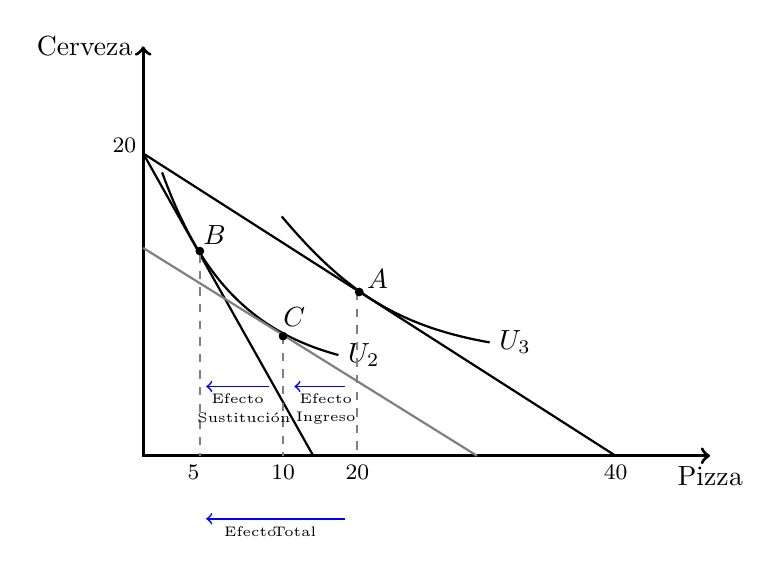
\begin{tikzpicture}[scale=0.8]
\draw[very thick,<->] (0,6.5) node[left]{Cerveza}--(0,0)--(9,0) node[below]{Pizza};
\draw [thick] (2.2,3.8) to [out=310,in=170] (5.5,1.8);
\node [right] at (5.5,1.8) {$U_3$};
\draw [thick] (0.3,4.5) to [out=290,in=165] (3.1,1.6);
\node [right] at (3.1,1.6) {$U_2$};
\node[below] at (3.4,0) {\footnotesize 20};
\node[below] at (7.5,0) {\footnotesize 40};
\node[below] at (-0.3,5.2) {\footnotesize 20};
\node[below] at (2.22,0) {\footnotesize 10};
\node[below] at (0.8,0) {\footnotesize 5};
\draw [thick] (0,4.8) -- (7.5,0);
\draw [thick] (0,4.8) -- (2.7,0);
\draw[thick, dashed,gray](0.9,3.2)--(0.9,0);
\draw[thick, dashed,gray](3.4,2.6)--(3.4,0);
\draw[thick, dashed,gray](2.22,1.9)--(2.22,0);
\draw [thick, gray] (0,3.3) -- (5.3,0);
\draw[semithick, blue, <-] (1,-1)--(3.2,-1);
\node[] at (1.7,-1.2){\tiny Efecto};
\node[] at (2.4,-1.2){\tiny Total};
\draw[semithick, blue, <-] (2.4,1.1)--(3.2,1.1);
\node[] at (2.9,0.9){\tiny Efecto};
\node[] at (2.9,0.6){\tiny Ingreso};
\draw[semithick, blue, <-] (1,1.1)--(2,1.1);
\node[] at (1.5,0.9){\tiny Efecto};
\node[] at (1.6,0.6){\tiny Sustitución};
\node [above] at (2.4,1.9) {$C$};
\draw[fill] (2.22,1.9) circle [radius =0.06];
\node [right] at (0.8,3.5) {$B$};
\draw[fill] (0.9,3.25) circle [radius =0.06];
\node [right] at (3.4,2.8) {$A$};
\draw[fill] (3.43,2.6) circle [radius =0.06];
\end{tikzpicture}
\end{center}
\end{figure}
\end{center}
\end{frame}


\end{document}

